%%% template.tex
%%%
%%% This LaTeX source document can be used as the basis for your technical
%%% paper or abstract.

%%% The parameter to the ``documentclass'' command is very important.
%%% - use ``review'' for content submitted for review.
%%% - use ``preprint'' for accepted content you are making available.
%%% - use ``tog'' for technical papers accepted to the TOG journal and
%%%   for presentation at the SIGGRAPH or SIGGRAPH Asia conference.
%%% - use ``conference'' for final content accepted to a sponsored event
%%%   (hint: If you don't know, you should use ``conference.'')

\documentclass[tog]{acmsiggraph}

\usepackage{balance}  % to better equalize the last page
\usepackage{graphics} % for EPS, load graphicx instead
\usepackage{times}    % comment if you want LaTeX's default font
\usepackage{url}      % llt: nicely formatted URL

\usepackage{todonotes} % add notes in th paper

% llt: Define a global style for URLs, rather that the default one
\makeatletter
\def\url@leostyle{%
  \@ifundefined{selectfont}{\def\UrlFont{\sf}}{\def\UrlFont{\small\bf\ttfamily}}}
\makeatother
\urlstyle{leo}

%%% Make the ``BibTeX'' word pretty...

\def\BibTeX{{\rm B\kern-.05em{\sc i\kern-.025em b}\kern-.08em
    T\kern-.1667em\lower.7ex\hbox{E}\kern-.125emX}}

%%% Used by the ``review'' variation; the online ID will be printed on 
%%% every page of the content.

\TOGonlineid{45678}

%%% Used by the ``preprint'' variation.

\TOGvolume{0}
\TOGnumber{0}

\title{Introducing postural variability improves the distribution of muscular loads during mid-air gestural interaction}

\author{
  Anonymous N. Hidden\thanks{e-mail:anonymous@cs.somewhere.edu}\\Department, Institution, location}
\pdfauthor{Anonymous N. Hidden}

\keywords{
	Mid-air interaction; 3D interaction; Gorilla arm; comparative study; physical ergonomics; user performance; optical motion capture; biomechanical simulation.
}

\begin{document}

%%% This is the ``teaser'' command, which puts an figure, centered, below 
%%% the title and author information, and above the body of the content.

\teaser{
%\begin{figure}%[tbh]
\centering
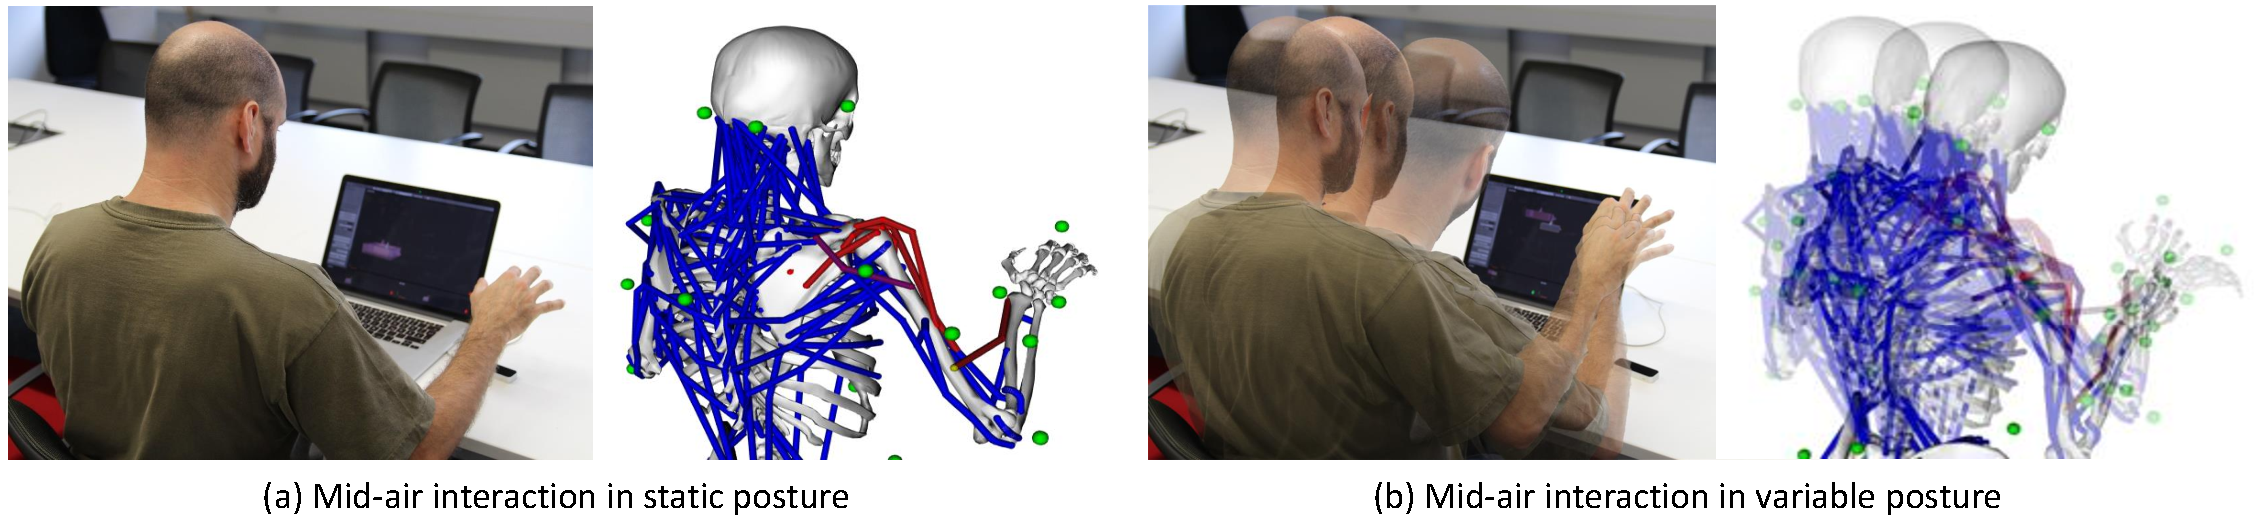
\includegraphics[width=\textwidth]{img/moneyshot}
\label{fig:moneyshot}
\caption{This paper analyses the effect of posture variability of upper body on muscular fatigue and the casually called ''Gorilla arm´´ effect. Motion capture-based biomechanical simulation was used to understand differences in joint loads, muscle forces and activations. This figure shows the two conditions which we studied: in static posture the load is all the time concentrated on the same muscles and they quickly get fatigued, in variable posture the loaded muscles change over time which gives more time for them to recover.}
%\end{figure}
} 

\maketitle

\begin{abstract}


Only time will tell if motion-controlled systems are the future of gaming and other industries and if mid-air gestureal input will eventually offering a more intuitive way to play games, learn certain skills and more.

If mid-air gestural input is promised to become a widespread input modality, it is necessary to assess its ergonomics and propose design guidelines which will guarantee a safe usage of mid-air gestures in the long run. This paper presents how muscular fatigue and the resulting ``Gorilla arm'' effect during mid-air interaction can be mitigated by introducing additional variability of the whole upper body posture. This paper also introduces an indirect pervasive strategy leveraging head-tracking and parallax effect encouraging postural changes during the interaction. A user study involving 30 subjects validates the setup through quantitative analysis and qualitative analysis. A quantitative analysis was conducted on data obtained using an optical motion capture setup together with biomechanical simulation. A qualitative analysis was conducted through Questionnaires. Both questionnaires and musculoskeletal loads data support our hypothesis and shows a statistically significant 15-25\% decrease in average muscle loads on the anterior and medial deltoids and biceps long  in the modified condition comparing to the baseline.
\end{abstract}

\begin{CRcatlist}
  \CRcat{H.5.2.}{Information Interfaces and Presentation (e.g. HCI)}{User Interfaces};
%  \CRcat{I.X.X}{Animation}{Inut method}{Radiosity};
\end{CRcatlist}

\keywordlist

%% Required for all content. 

\copyrightspace

\section{Introduction}

Since the advent of multitouch enabled smartphones, multi-touch input has become a ubiquitous input modality. Recent development and advances in acquisition devices and computer vision have today the potential to empower users with novel interaction modalities referred as mid-air gestures and depicted in Figure 1. %~\ref{fig:moneyshot}.
If mid-air gestural input is promised to become as widespread as multitouch touch gestural input, it is necessary to conduct the ergonomic studies and to provide a set of relevant design guidelines which will guarantee a safe and optimal user experience.

Even if the literature in the field of biomechanics states that a prolonged solicitation of certain muscles and joints leads to chronic pain and even functional disability \cite{franklyn-miller_biomechanical_2014}, the impact of an extended usage of mid-air gestural input on the musculoskeletal system is yet to be known in a principled manner.  In the field of Human Computer Interaction, it has been observed that a prolonged interaction with a mid-air gesture interface might lead to a feeling of heaviness in the upper limb casually referred as \emph{gorilla-arm} \cite{aigner_understanding_2012}. If many studies have already assessed both the ergonomics and the performance of mid-air gesture \cite{aigner_understanding_2012,hincapie-ramos_consumed_2014,bachynskyi_performance_2015,sridhar_investigating_2015,straker_comparison_2008}, only a few design guidelines have been suggested. Ramoe et al. suggested to limit the amount of time spent by the user while raising her/his arm \cite{hincapie-ramos_consumed_2014}. Aigner et al. highlighted the influence of pointing as well as iconic bimanual gestures \cite{aigner_understanding_2012} on both usability and performance. Kim et al. analyzed smartphone interaction and found that body posture affects the range of motion and muscle activity of the thumb \cite{kim_biomechanical_2012}. They conclude that deeper analyses of ergonomics should be conducted in future work and do not provide any insight on how an interface designer could persuade users to adopt correct postures. We could not, however, find any guideline specifically addressing the interplay between interaction design and ergonomics. In this paper, we introduce and assess the following principle:~ \emph{``encouraging the user to deploy a large variety of muscles during the interaction''}. Our hypothesis is the following: ``A subject who often changes his upper body posture exhibit a broader muscle recruitment. When more muscles are involved in the interaction, each muscle undergoes less strain''. Applying this principle to mid-air gesture interaction should result in an input method with a well-balanced distribution of the muscular load, leading to less muscular strain and higher comfort.

While this guideline suits both touch and mid-air gestural input, it is currently assessed in the particular context of mid-air gesture interaction where the task consists of docking 3D objects. During the task, a persuasive interaction design leveraging both head tracking and parallax shift persuades the user to move his head and therefore change his upper body posture according to our guideline. Using a similar methodology as the one presented in \cite{bachynskyi_performance_2015}, we use optical motion capture, force plate sensors and biomechanical simulation to compute several indices of ergonomics. The use of biomechanical simulation not only provides a rich description of biomechanical events in the body, but it also overcomes the challenges posed by traditional ergonomics instruments such as goniometers and surface EMG.
To assess our hypothesis we perform a 40-participant comparative user study for a 3D docking task to compare pure mid-air gestural interface against mid-air gestural interface with enforced upper-body movements.
During the experiment, we record optical motion capture, which serves as input for biomechanical simulations computing a variety of indices from inside the body, including joint moments, muscle forces and recruitment. Our contribution consists of showing how introducing additional variability of the whole upper body posture has the potential to reduce muscular fatigue and the resulting ``Gorilla arm'' effect during mid-air interaction. We also we introduce and evaluate a persuasive interaction design leveraging head-tracking and parallax effect encouraging postural changes during the interaction.
 % easier to collaborate when paper is split between multiple files

\section{Experimental Method}

\subsection{Interaction Design}

\begin{figure}
\centering%
\includegraphics[width=\columnwidth]{img/user-setup}
\caption{A subject performing the docking task.}%
\label{fig:user-setup}
\end{figure}

Figure \ref{fig:user-setup} shows a picture of a user while accomplishing a \emph{docking task} \cite{zhai_quantifying_1998}, in which the subject has to use his hand to ``grab'' an object visualized in a virtual space and drop it inside a container. This task has been selected in order to lead the user to perform a set of long-lasting operations with mid-air hand movements. In the proposed setup, the subject can not accomplish the task while positioning the elbow on the surface of the desk. As in mid-air gesturing and interaction with large screens, this configuration is known to lead to muscular pain in the shoulder region (aka gorilla arm effect) \cite{hincapie-ramos_consumed_2014}.

The docking task is known to be better accomplished in presence of additional cues for the perception of depth, such as stereoscopic view \cite{boritz_study_1998}, or parallax effect \cite{Ware:1993:FTV:169059.169066}.
In order to encourage the user to involve upper body movements in the task, the movement of the head is tracked using the laptop's webcam and the inferred location of the head is used to change the viewpoint of the virtual 3D scene. The assumption is that, with parallax effect, users would have a tendency to change their stance in order to get different points of view and a better perception of depth, making the docking task easier.


\subsection{Apparatus}
The docking task has been performed on a 15 inches laptop (resolution 2880x1800, 2.4 GHz Intel Core i7, 16GB Ram).
The movement of the hand performing the docking task was tracked by a Leap Motion\footnote{\url{https://www.leapmotion.com/} -- September 25th, 2015}, whose programming interface allows for the report of pinch gestures.

The experiment was performed in a MoCap laboratory. The motions of the users were recorded at 480Hz and with 1/2mm accuracy by PhaseSpace Impulse\footnote{\url{http://www.phasespace.com/} -- September 25th, 2015} system with 12 cameras. Thirty-height active markers were distributed on the whole body of user and were attached according to anatomical landmarks to a skin-tight suit. 
External forces acting on participants body were recorded at 125 Hz with accuracy 99.8\% by a chair instrumented with 8 force sensors: 2 under the seat, 1 under backrest, 2 under armrests, 1 under footrest and 2 under movable force plates. 
The MoCap and force data were recorded by a single high-end machine (Dell Precision M4800) and synchronized with the task machine through network (\textless 1ms latency).


\subsection{Task}

\begin{figure*}%[tb]
\centering%
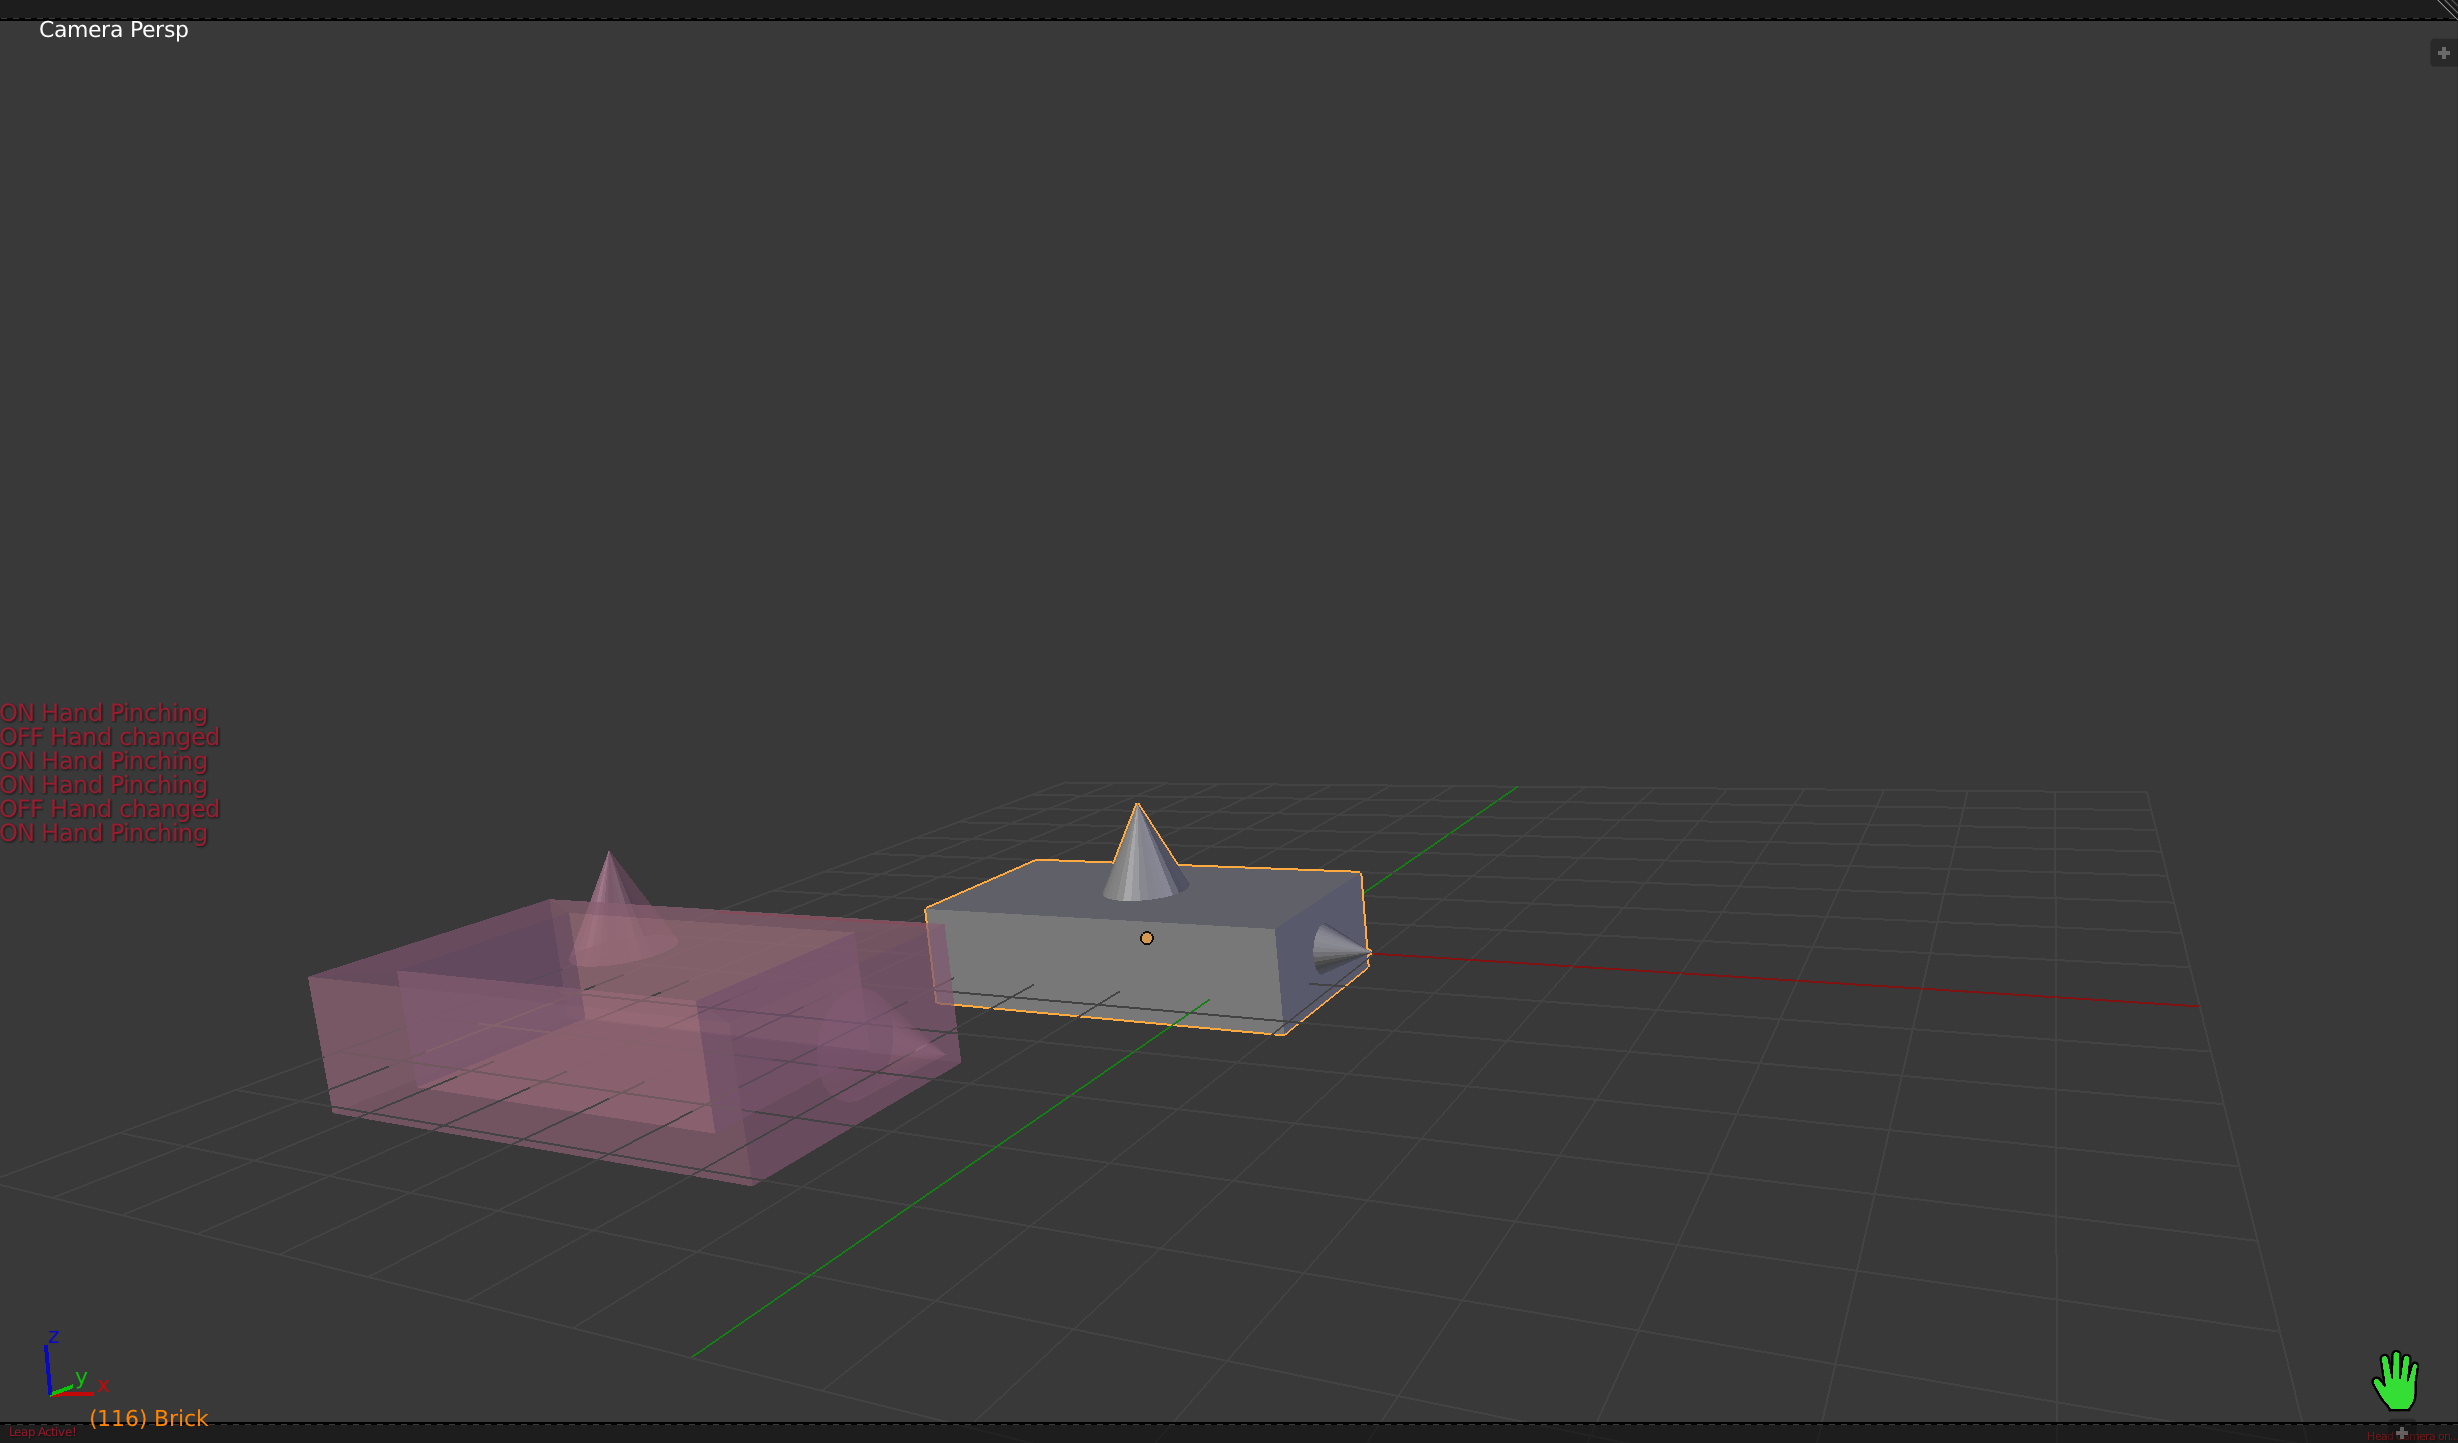
\includegraphics[width=\columnwidth]{img/task-performing-crop}
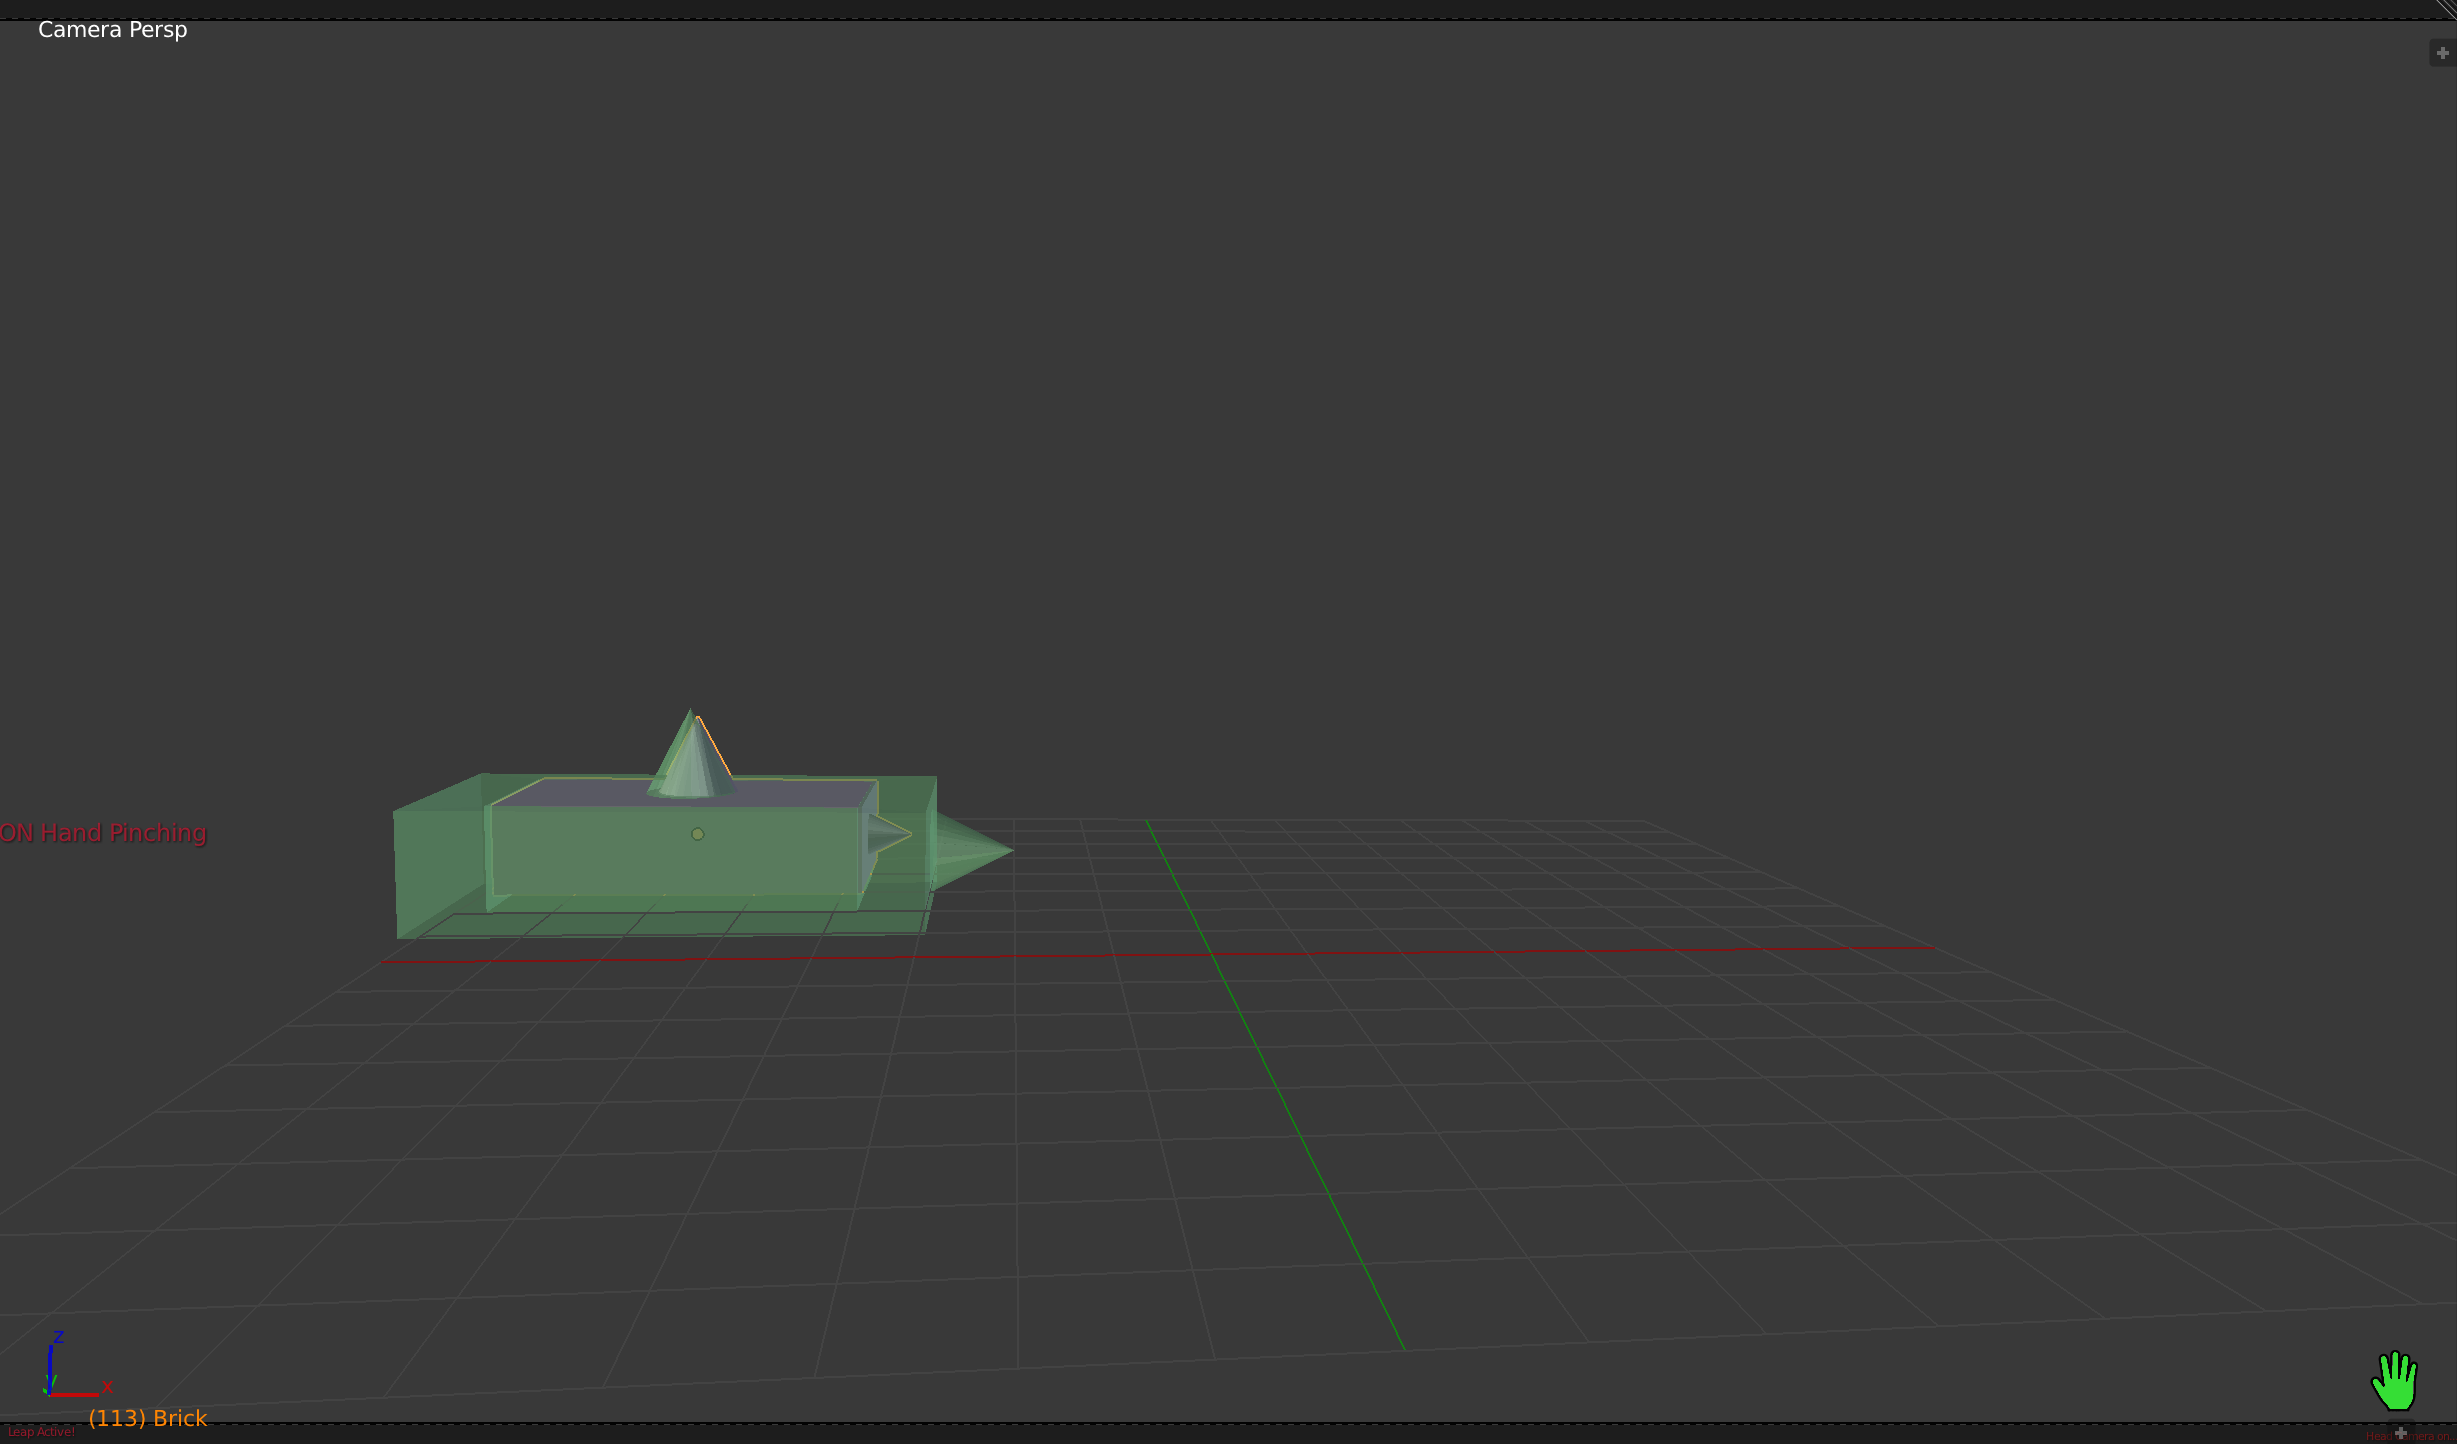
\includegraphics[width=\columnwidth]{img/task-accomplished-crop}
\caption{Two screenshots of the docking task as visualized on the laptop provided to the subjects. Left: the user is dragging the object inside the container. Right: the object has been correctly placed inside the container.}%
\label{fig:task-screenshots}
\end{figure*}

Figure \ref{fig:task-screenshots} shows two screenshots of the task as visualized on the screen of the laptop provided to the subject. Each trial consisted of docking a grey box inside a bigger semi-transparent red box in the virtual 3D scene (Figure \ref{fig:task-screenshots}, left).
As visual cue for the accomplishment of the task, when the grey box was correctly docked, the semi-transparent red box turned green (Figure \ref{fig:task-screenshots}, right).
In order to start the dragging procedure, the users had first to position their hand in the visibility zone of the hand-tracker and then ``pinch'' the virtual object by joining the tips of the index and the thumb. At this point, the movement of the hand in the tracking space is translated into a movement of the box in the virtual 3D scene. Users could drag the object into the container and release it by un-pinching it, i.e., separating the index and the thumb.

At the beginning of each trial, the grey object was always positioned at the center of the virtual scene, while the position of the red container was randomly selected by the system among eight fixed locations.
There was no limit to the number of times the object could be dragged and released in order to dock it correctly. It means that several drags can be performed to reach the goal.
When the trial was accomplished, the system was automatically switching to the next trial after 2 seconds.

\subsection{Experimental Design}

The docking task has been conducted on two conditions: Baseline (B) and Head Tracking (HT). In the B condition the virtual camera was fixed. In the HT condition the movement of the users' head in the real world controlled the position of the virtual camera, thus allowing for a parallax effect.
The subject had to perform as many docking operations as possible in 15+15 minutes (B + HT conditions). 
\todo[inline]{Here. We have to finally justify why we did not counterbalance. A proposal follows. Please, check-it -- FN}
The conditions have not been counterbalanced in order to present the users with a progression in the complexity of the interaction paradigm. This need emerged from the observation of the interaction of the first subjects. In the B conditions users take confidence with the gesture-based object manipulation system; in the HT condition they add the head control to the interaction.
The lack of counter-balance is a limit in the evaluation of the performances of the users in the docking task. However, since the experiment focuses on the measurement of the distribution of effort rather than of the effectiveness of the interaction method, precedence was given in effectively induce user to perform extra body movement.


The goal of the study is to measure if the stress on the shoulder reduces when the user increases the movement of the upper body.
Hence, as dependent variables we measured the quantity of movement of the head in space and a set of biomechanical indices described in detail in a later section.
\todo[inline]{or maybe now. Let's see.}
Additionally, we measured the trial completion time and the number of tasks accomplished to verify if the performance of the docking increased thanks to the parallax effect.


\subsection{Software Material}

The software driving the experiment has been programmed inside the Blender 3D authoring tool\footnote{\url{http://www.blender.org/} -- July 12th, 2016}. The task generator, the code allowing the manipulation of the 3D objects using the Leap Motion, and the logging system have been developed by the authors as Blender add-on.

In the virtual scene, the size of the box was set to 4x2x1 units, the external size of the container was set to 5,6x2,8x1,4. The location tolerance was set to 0.6 units (15\% of the longer edge) and has been imposed by the authors according to preliminary tests. At each trial, the initial position of the grey object is alway the origin of the axes, while the position of the target container is chosen randomly from 8 possible positions, given by the combination of the following translations: horizontal $\pm 6$, vertical $\pm 4$, depth $0$ or $6$.
The virtual camera is positioned at the point $0,-15.5,5.4$ and looks at the vertical axis with a rotation of 10 degrees towards the surface.

When enabled, the movement of the virtual camera is driven by the position of the face of the user. The face position is recognized through an analysis of the image captured by the webcam of the laptop. The face is recognized via a custom made application, developed in Processing\footnote{\url{https://processing.org/} -- July 12th, 2016}, which takes advantage of the OpenCV library\footnote{\url{http://opencv.org/} -- July 12th, 2016}.

% Movement proportions
%Face position is normalized
%At 60cm distance from the screen --> 20 cm on a side --> 0.5 units.
%Rotation was set to 120 degrees, it means that 0.5 on one side translates into 60 degs.
% it means that +/- 10 cm translates into +/- 30 degs rotation
%The rotation point is at 15 in front of the camera, almost around the original vertical axis.
The movement of the camera is accomplished by mapping the relative position of the face inside the webcam view to a rotation of the camera around a point in space.
After some preliminary test, the mapping was set to translate about $\pm 10cm$ of translation of the head into $\pm 30deg$ of rotation of the camera around a point set 15 units at the front (hence, close to the vertical axis).

%\todo[inline]{Actually this setup amplifies the rotation of the virtual camera with respect to a faithful simulation of the reality. It is more convenient for the user because he need less head movement to perform the same rotation, but it penalizes the experiment since it requires less motion from the user. We did not think about it in time. What to do? Skip details? - FN}

\subsection{Participants}

% code in file QuestionnaireAnalysis-RProj/analyse_profiles.R

A total of 40 subjects were recruited for the study. The data collected from the first eight subjects has been discarded because the software was still in a fine-tuning phase. Two left-handed users were discarded from the data analysis in order to focus the computation on the average stress of the muscles of the same arm. Hence, the results presented in the rest of the paper consider 30 subjects (10 Female, 20 Male), 25.53 years old on average (min=19, max=39, SD=3.91). Most of the subjects were university students in computer science.
The experiment was advertised on social networks and university mailing lists. There were no ethical issues involved in the experiment. Each participant received 10 Euros for one hour of availability, which included the time needed to wear the suit on which the markers are attached, to calibrate the motion capture, and to run the experiment.


\subsection{Procedure}

Users were sitting on a chair in front of an office desk. The chair was equipped with pressure sensors on the seat, the back, and the arm rests. Other pressure sensors were positioned on the floor, under the feet, and over the desk, under the hands. Thus we have recorded all external forces acting on a user. The laptop was positioned over the desk, in front of the user. The leap motion was positioned on the right side of the laptop in the place where typically mouse is used. However, both the laptop and the Leap were moved farther from the user, preventing the user from holding the elbow on the pressure sensor while operating mid-air gestures.
An operator assisted the users to take a comfortable position and to give instructions. Users had between two-five minutes to try the system and ask questions to the operator.
During the accomplishment of tasks, in order to avoid any disturbance, the operator was sitting about 4 meters behind the user.


\section{Analyses}
To extract musculoskeletal loads and muscle usage we performed extensive processing of the data collected in the experiment. We applied the typical processing to prepare the motion capture data for biomechanical simulation and user performance modeling as described in the previous works within HCI as well as in biomechanics \cite{kontaxis2009framework,bachynskyi_performance_2015}.
The processing consisted of 3 stages: \\
\textbf{Preprocess} the data for biomechanical simulation and performance modeling by removing occlusions and reflections, interpolation of missing regions and removing noise by Kalman filter.\\
\textbf{Extract user performance} data, integrate it with quantitative measures and segment the data into timeperiods of individual tasks.\\
\textbf{Perform biomechanical simulation} on the data to extract physiological loads and muscle recruitment. As described in previous work \cite{bachynskyi_performance_2015,opensim}, biomechanical simulation consists of multiple pipelined steps: 
\begin{itemize}
\item \textbf{Model scaling} adjusts model segments size and mass distribution to match the parameters of a subject,
\item \textbf{Inverse Kinematics} computes \textbf{generalized coordinates} at all joints for each timeframe,
\item \textbf{Inverse Dynamics} computes \textbf{moments at joints} based on the generalized coordinates, and
\item \textbf{Static Optimisation} resolves moments at joints to the moments induced by individual muscles, \textbf{muscle forces and activations}, assuming movement optimality with respect to muscular strain.
\end{itemize}
To run biomechanical simulation we used OpenSim software \cite{opensim} and state-of-the-art musculoskeletal model of the full body\footnote{\url{http://www.musculographics.com/html/products/fullbodymodel.html} -- September 25th, 2015} \cite{holzbaur2005model}. The outputs of biomechanical simulation have been validated in multiple previous works against direct measurements of joint angles, estimations of joint moments or electromyography recordings \cite{bachynskyi2014motion}. The biomechanical simulation provides moments for 109 joints of the full body. Due to computational reasons muscle forces and activations were computed for 148 muscles of the body part above pelvis.\\
\textbf{Perform analysis} and statistical hypothesis testing of the dataset. We use MATLAB, R, Microsoft Excel and visualizations in MovExp \cite{palmas2014movexp} to analyze the data and inspect the results. We start by analysis of visualizations to identify patterns within the dataset. Then we investigate statistical distributions of variables and visually inspect them for normality. We perform Shapiro-Wilk normality tests to verify for a normal distribution of the data. If the data distribution is normal, we perform paired t-tests to identify statistical effects, otherwise Wilcoxon signed-rank tests are used.

\section{Results}

We have analysed more than 400 dependent variables. In this section we report the results for variables which showed a statistically significant difference between the B and HT conditions. The full table is provided as a supplementary material. 
The variables are divided in five groups: movement of the head in space, users' performance and self-assessment, joint moments, muscle forces, and muscle activation.

\subsection{Movement of the head}

% code in file QuestionnaireAnalysis-RProj/analyse_head_movement2.R

\begin{figure}[tb]
\centering%
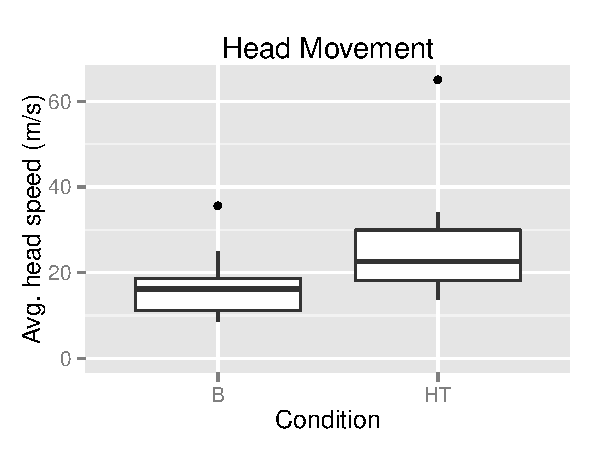
\includegraphics[width=\columnwidth]{img/HeadMovement-ggplot}%
\caption{Subjects' head average speed in the two conditions.}%
\label{fig:head-movement}
\end{figure}

This section describes how we verified that the parallax effect effectively induced the subjects to increase the movement of their head. We considered the the motion of the head as captured by the motion capture system. More precisely, we extracted the x, y, z motion coordinates of the marker positioned over the right eye. For each user, and separately for the B and HT conditions, we integrated the traveled path and normalized it by the time spent in accomplishing the task. The result is the average speed of the head during a task in a given condition.

Between trials, subjects were often observed to sit back on the chair in order to relax or discuss with the operator. In so doing, they were performing wide head movements which were not functional to the accomplishment of the task.
Hence, the motion has been considered only for the time spent between the actual beginning of a trial, when the user first pinched the object, and its accomplishment, when the user performed the last drop in the target container.
The measured head average speed is 16.21 m/s (SD=5.95) for the B condition and 24.51 m/s (SD=9.89) for the HT condition (see Figure \ref{fig:head-movement}).

A Shapiro-Wilk normality test showed that the distribution of speeds in the B condition is normal (p=0.0117), but not for the HT condition (p~\textless~0.001). Hence we measure the statistical difference in the two conditions using a Wilcoxon signed rank test. Results show a statistically significant difference in the average speed in the two conditions (V=23, p~\textless~0.001).
We can hence hence assume with 99.9\% confidence that the parallax effect indeed invited the users to perform head movements on average 51.17\% wider than without tracking.


\subsection{User performance and subjective measures}


% questionnarie
After the experiment, subjects were asked to fill a questionnaire to self-assess how much they liked the interface and how much pain in the shoulder they felt after the first and after the second task.

% liked the interface?
% QuestionnaireAnalysis-RProj/analyse_F.R
% QuestionnaireAnalysis-RProj/analyse_C.R
Twenty-three out of the thirty subjects answered the question: ``How did you find the interaction overall?", on a scale from 1 (bad) to 6 (good). The results reported in the following table (M=4.48, SD=0.89).

%appreciation
% 1  2  3  4  5  6 
% 0  1  1  9 10  2 

\begin{center}
\begin{tabular}{ | c | c | c | c | c | c | c | }
\hline
& bad & \ldots  & \ldots & \ldots & \ldots & good \\
\hline
Vote & 1 & 2 & 3 & 4 & 5 & 6 \\
\hline
Count & 0 & 1 & 1 & 9 & 10 & 2 \\
\hline
\end{tabular}\end{center}

Twenty-height out of the thirty subjects answered Yes or No on the question: ``Did you find useful the camera movement?''. Nineteen subjects (67.86\%) answered Yes.
Together with the previous results it indicates an overall good appreciation of the interaction method.

% QuestionnaireAnalysis-RProj/analyse_performance.R
% Performance (avg observation duration==docking time)
Subjects performed an average of 63.97 docking operations (SD=21.53) in the B condition and an average of 68.07 (SD=22.47) in the HT condition.
In terms of average time needed to accomplish a docking trial, the results are 12.72 secs (SD=8.45) for the B condition and 11.66 seconds (SD=5.54) for the HT condition.
% t.test w/ respect to conditions
A paired Wilcoxon signed rank test shows that there is no significant difference between the average time needed by a user to accomplish a docking trial between the B and the HT conditions (V=152, p=0.0998).


% Borg self-assessment for pain
% QuestionnaireAnalysis-RProj/analyse_borg.R
We observed that most of the subjects reported a slight pain in the shoulder already after the first condition. It is coherent with the self-assessment reported in the questionnaires.
Twenty-three out of the thirty subjects did a self-assessment of the pain perceived in their arm after the first and the second conditions, i.e., after 15 minutes and after 30 minutes. The assessment is based on the Borg RPE (Rate of Perceived Exertion) scale \cite{borg_borgs_1998}.
The Borg scale ask subjects to self-assess the perceived pain on a scale from 6 (no exertion at all) to 20 (maximal exertion).
After the first 15 minutes, subjects reported an average perceived pain of 11.93 points (min=6, max=19, SD=2.76). At the end of the second condition, after 30 minutes, the subjects reported an average of 11.34 points (min=6, max=16, SD=2.76).
In both conditions, the Borg scores follow a normal distribution. A paired t-test shows that there is no statistical difference in the perceived level of pain between the two conditions (t(22)=1.45, p=0.1622).
It means that the pain felt by the users has been provoked within the first 15 minutes of use of the interface, and the perceived pain remained stable until the 30th minute.


\subsection{Joint moments}

\begin{figure}[tb]
\centering%
%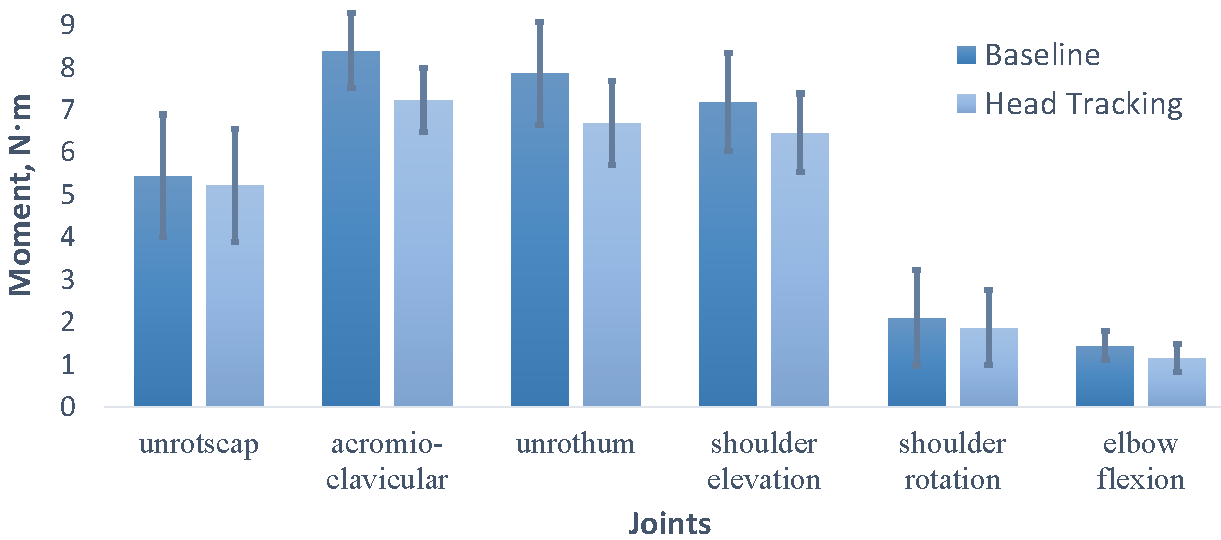
\includegraphics[width=\columnwidth]{img/ShoulderJointMoments1}%
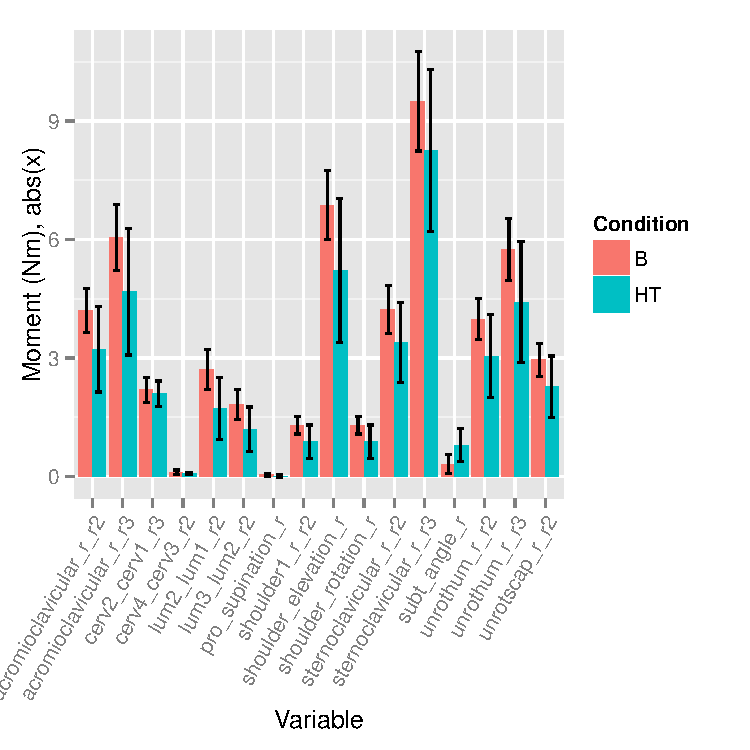
\includegraphics[width=\columnwidth]{img/Moments}%
\caption{The joints' degree of freedom whose moment magnitude changed significantly between B and HT conditions. Vertical bars denote 95\% confidence intervals.}%
\label{fig:moments}
\end{figure}

The moment magnitude (measure in Newton per meters) exerted at each joint has been measured with 103 variables. Each variable represent a degree of freedom of a joint. Each joint is modelled with one to three degrees of freedom.
A significant difference of the moments between B and HT conditions is present in 16 variables.
As can be observed in Figure~\ref{fig:moments}, the average magnitudes of 15 out 16 joint moments is decreased in head tracking condition comparing to the baseline by 4.2\%-19.9\% depending on a joint. There were significant differences for elbow flexion moment between HT (M=1.16, SD=1.37) and B (M=1.45, SD=0.59) conditions, t(29)=2.10, p=0.05; for sternoclavicular moment between HT (M=10.178, SD=3.86) and B (M=10.381, SD=3.56), t(29)=1.91, p=0.07. Unrotscapular, acromioclavicular, unrothumeral moments were less significant (0.1~\textless ~p~\textless~0.2) with differences between conditions 4.2\%, 13.8\% and 14.9\% respectively.

For unused upper extremity only slight increase in sternocalvicular moment is significant between HT (M=4.43, SD=2.95) and B (M=4.36, SD=2.57), t(29)=-1.69, p=0.1. The mean magnitudes of joint moments in lumbar and upper back and neck slightly decrease for most but 2 joints. The decreases in moments are significant for all neck joints (p~\textless~0.1), while the increases are not significant (0.2~\textless~p).
In the lower body there are significant increases by 8.1\% in hip moments t(29)=-1.76, p=0.09 and 22.7\% decrease in knee moments t(29)=1.89, p=0.07.



\subsection{Muscle forces}

\begin{figure}[tb]
\centering%
%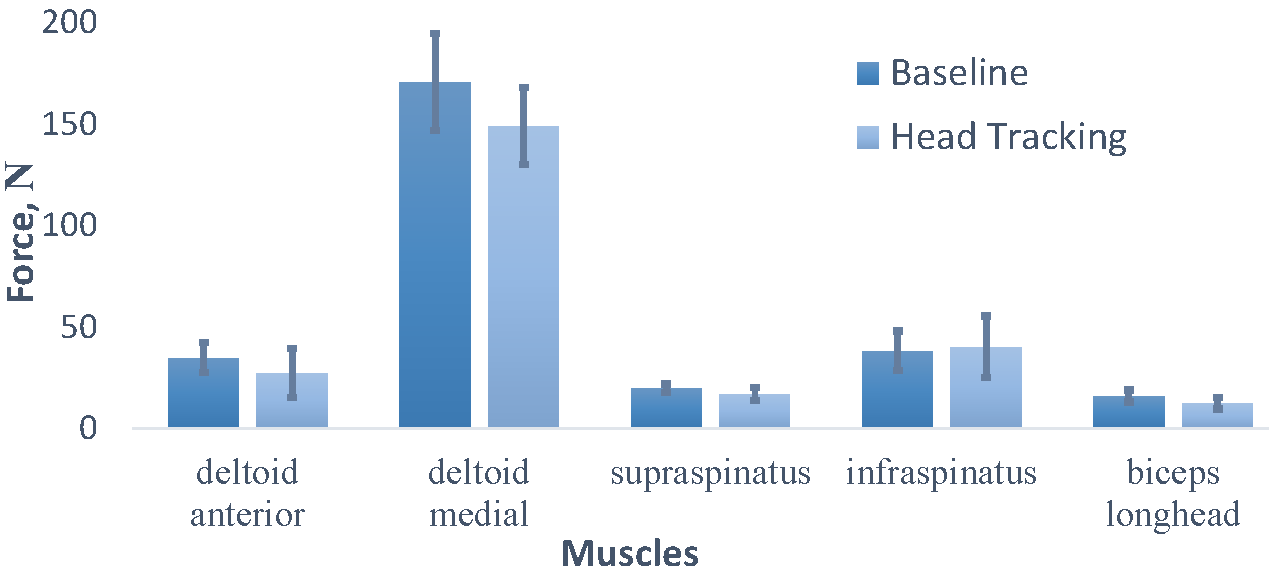
\includegraphics[width=\columnwidth]{img/MuscleForces}%
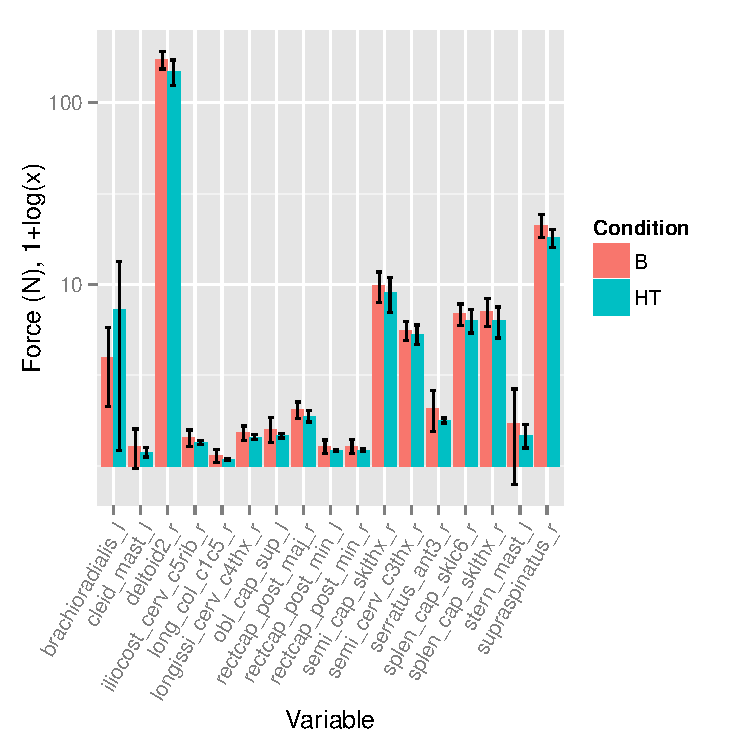
\includegraphics[width=\columnwidth]{img/Forces}%
\caption{The muscles whose exerted forces changed significantly between B and HT conditions. Vertical bars denote 95\% confidence intervals.}%
\label{fig:forces}
\end{figure}


As can be seen on Figures~\ref{fig:forces} and \ref{fig:activations}, muscle forces and activations demonstrate the same pattern in differences between the conditions.

\subsection{Muscle activations}

\begin{figure}[tb]
\centering%
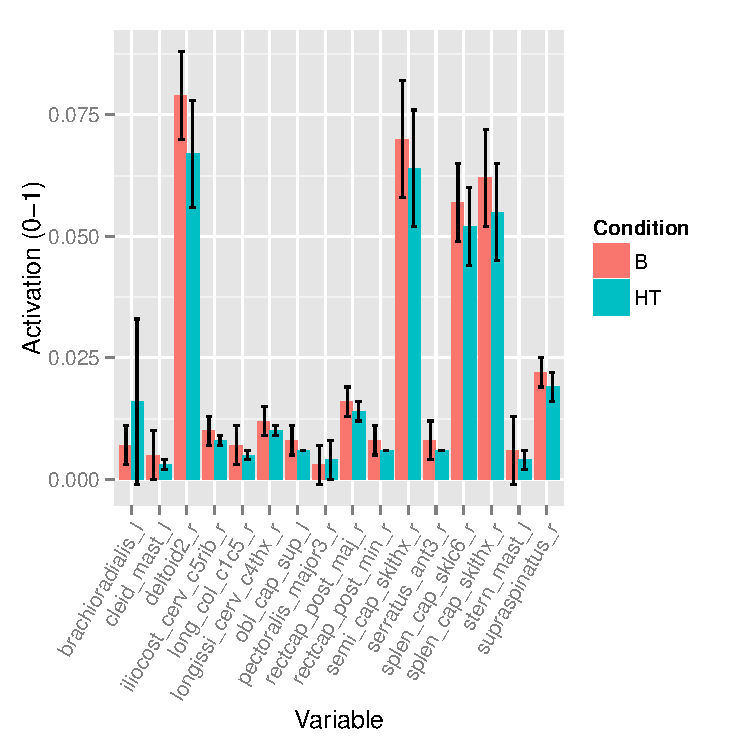
\includegraphics[width=\columnwidth]{img/Activations}%
\caption{
The muscles whose activation factor changed significantly between B and HT conditions. Vertical bars denote 95\% confidence intervals.}%
\label{fig:activations}
\end{figure}

 In the paper we provide values for the activations, as they roughly represent forces normalized by the size of each muscle and thus are considered on the same scale for all muscles. There are significant differences in activation of medial deltoid between HT (M=0.068, SD=0.031) and B (M=0.078, SD=0.025) conditions, t(29)=2.66, p=0.01; for supraspinatus: HT (M=0.019, SD=0.007) and B (M=0.022, SD=0.008), t(29)=2.05, p=0.05; and biceps longhead: HT (M=0.010, SD=0.006) and B (M=0.012, SD=0.006), t(29)=2.15, p=0.04. Less significant are differences for deltoid anterior: HT (M=0.012, SD=0.009) and B (M=0.015, SD=0.015), t(29)=1.52, p=0.14; for infraspinatus: HT (M=0.0164, SD=0.011) and B (M=0.0159, SD=0.016), t(29)=1.47, p=0.15; for brachioradialis: HT (M=0.009, SD=0.004) and B (M=0.010, SD=0.009), t(29)=1.38, p=0.18. To demonstrate the scale of the variable ``average activations'', the median for HT condition is 0.0055, and the median for the baseline is 0.0057.

There are no significant differences for muscle activations of lumbar region, but there are significant decreases by 7.3-15.7\% in activations of 2 upper back and neck muscles: splenius capitis and semispinalis capitis, (p~\textless~0.1). Multiple less recruited upper body muscles exhibit increase in their activation, however the increase is not significant.


\section{Discussion and conclusion}

\todo[inline]{Report even if the subjects performance did not change and muscular pain is perceived the same, since users in HT condition were indeed moving more the head their muscular effort in better distributed. This can be an advantage because pain is often perceived only the day after. - FN}

\todo[inline]{Speculations. The system can be used to analyse users behavior. Now offline, in future between gaming sessions or even in real-time. The data on the muscular effrt can be used in future sessions or in real time to fine tune the game parameters or suggest pauses. Of course the methodology can be used already now for design and testing. }

The study and the simulation results support the proposed ``postural variability'' principle for mid-air interaction.
The results show that posture variability decreases the recruitment of the muscles which are traditionally most loaded in mid-air interaction by 15-25\%. 
Surprisingly, the load on the neighbouring and postural muscles is in most, but very few cases also decreased, and the total load on all muscles is decreased as well.
Thus increasing postural variability decreases loads on the whole body and as a result should reduce fatigue and strain. 
This can be explained by the fact that in static posture the muscles have to be activated all the time and often agonists and antagonists are coactivated, while with variable posture the coactivation can be smaller.

The analysis of the Borg RPE self-assessment for pain conducted on the questionnaires revealed no significant differences between the two conditions (with or without head tracking) after 15 and 30 minutes of mid-air gesturing. This suggests that the experiments we conducted might not have had a sufficient duration (30 minutes) to exhibit a significant difference.
Our findings are currently limited to the single type of mid-air task, and to better generalize the ``postural variability'' principle future work has to test it on other types of mid-air tasks as well as on the tasks with touch screen interactions, or handheld devices.
The analysis conducted for this paper focused on the upper body. Future work will be conducted on the whole body in order to better understand the role of the hips and the lower limbs in the adaptation of the posture while working in sitting positions.


%\section*{Acknowledgements}
%To Robert, for all the bagels.

\bibliographystyle{acmsiggraph}
\nocite{*}
\bibliography{sample}
\end{document}
